\documentclass{BUP}
%%%%%%%%%%%%%%%%%%%%%%%%%%%%%%%%%%%%%%%%%%%%%%%%%%%%%%%%%%%%%%%%%%%%%%%%%%%
\newcommand\tab[1][1cm]{\hspace*{#1}} %% \tab komutu bir 1 cm boşluk bırakması sağlar.
\begin{document}
\shorthandoff{=}
\setlength{\headheight}{16pt} % "En az 16 olmalı" diye uyarı vermişti.
%Bölümler----------------------------------
\thispagestyle{empty} 
\begin{figure}[H]
\centering

\includegraphics[scale=0.2]{logomuz}
\end{figure}
\begin{center}
\textbf{T.C.}\\
\textbf{BİLECİK ŞEYH EDEBALİ ÜNİVERSİTESİ}\\
\textbf{MÜHENDİSLİK FAKÜLTESİ}

\textbf{BİLGİSAYAR MÜHENDİSLİĞİ BÖLÜMÜ}
\end{center}

\vspace*{4cm}
\begin{center}
\textbf{Bilgisayar Ağları}


\textbf{Ders Notu}
\end{center}

\vspace*{\fill}
\begin{center}
\textbf{öğretim Görevlisi : Sayın Murat ÖZALP}

\textbf{BİLECİK}\\ 
\textbf{\today}
\end{center}

\pagenumbering{roman}
\setcounter{page}{2}
\tableofcontents%bu komutun olduðu yerde içindekiler oluþturulur.
\renewcommand*\listfigurename{\centerline{\bf\normalsize ŞEKİL LİSTESİ}}
\listoffigures%bu komutun olduðu yerde þekiller listesi oluþturulur
\addcontentsline{toc}{section}{ŞEKİL LİSTESİ}
\renewcommand*\listtablename{\centerline{\bf\normalsize TABLO LİSTESİ}}
\listoftables%bu komutun olduğu yerde tablolar listesi oluşturulur
\addcontentsline{toc}{section}{TABLO LİSTESİ}
%\renewcommand{\centerline{\textbf \normalsize ŞEKİL LİSTESİ}}
\begin{center}
    \textbf{TEŞEKKÜR}
\end{center}
Bu çalışma, 2022 yılında BŞEÜ Bilgisayar Mühendisliği 4. sınıf öğrencilerinin önerisi üzerine başlatılmıştır. El yazısı ile yazılmış ve eski kalmış olan ders notlarının kolay güncellenmesi ve güncel tutulması amacını taşımaktadır.

\textbf{Katkıda bulunanlar:}
\begin{itemize}
    \item İbrahim Khalil Atteib Yacoub
    \item Aleyna Çelik
    \item ...
\end{itemize}
\pagenumbering{arabic}
\setcounter{page}{1},
\pagestyle{fancy}
\renewcommand{\footrulewidth}{0.4pt}% Default \footrulewidth is 0pt
\fancyfoot[C]{\thepage\ / \pageref{LastPage}}
\section{GİRİŞ}
Bu çalışma, 2022 yılında BŞEÜ Bilgisayar Mühendisliği 4. sınıf öğrencilerinin önerisi üzerine başlatılmıştır. El yazısı ile yazılmış ve eski kalmış olan ders notlarının kolay güncellenmesi ve güncel tutulması amacını taşımaktadır.

\textbf{Katkıda bulunanlar:}
\begin{itemize}
    \item İbrahim Khalil Atteib Yacoub
    \item Aleyna Çelik
    \item ...
\end{itemize}
\section{OSI MODELİ (OSI KATMANLARI)}

\subsection{Katmanlar}

\subsubsection{Fiziksel Katmanlar}

Birinci katman donanımları:
\begin{enumerate}
\item Bakır ve FiberOptik Kablolar
\item RF (Antenler)
\item Sınyali 
\item Kablosuz iletişimde kullanlan Hava 
\end{enumerate}

\subsubsection{Veri Bağı Katmanı}


\subsubsection{AĞ Katmanı (IP) }

\subsubsection{Taşıma Katmanı}

\subsubsection{Uygulama Seviyesi Katmanları}


\section{TEMEL KAVRAMLAR}

\section{İLETİM ORTAMLARI}
Temelde atmosfer ve kablo olmak üzere iki farklı iletim ortamı mevcuttur.Atmosfer rf(radyo frekans) dalgalarını kullanarak  iletişim gerçekleşir.
Kablolarda ise genellikle fiberoptik ve bakır kablo kullanılmaktadır.

\subsection{İKİ TELLİ BAKIR TELEFON HATTI }
Telefon iletişimini sağlamak için tasarlanmıştır.Temel band ve geniş band internet hizmeti verilmektedir.
Analog modülasyon teknikleryle en fazla 56 k b/s'lik band genişliği sağlar.xDSL teknolojileriyle 25 M b/s'lik band genişliğine ulaşmaktadır.  
%\begin{figure}[!ht]
  %  \includegraphics{images/ikitellibakırkablo}
  % \caption{İki telli Bakır Kablo}
  %  \label{fig:iki_telli_bakir_kablo}
 %\end{figure}

 \subsection{KOOKSİYEL(CCOKSİAL)KABLO}
 Genellikle elektiriksel gürültünün yoğun olduğu şartlarda kullanılırdı.Yalıtkan bir tüpün içerisinde  giden bir tel ve tüpün dışına sarılmış kafes şeklinde teller vardır.
 Yerel ağlarda (LAN) 180m'de(max) 10M b/s bant genişliği sağlar.Bu kullanımı 10 Base 2 olarak bilinir.Daha sonra 500 m mesafede çalıştırılacak hale getirilir. 10 Base 2 ismiyle standartlaştırılmıştır.50 ohm'luk direnç değeri vardır.
 BNC tarzında connectörler kullanılır.Günümüzde LAN'da hiç kullanılmamaktadır.Sebebi hem 1o M b/s  hızının çok düşük olması,hem de UTP kablolar kadar ekonomik ve işlevsel olmamasıdır.
 Bilgisayr ağlarında doğrusal (bus) topolojilerde kullanılmıştır. 
 %
  %\begin{figure}[!ht]
  %   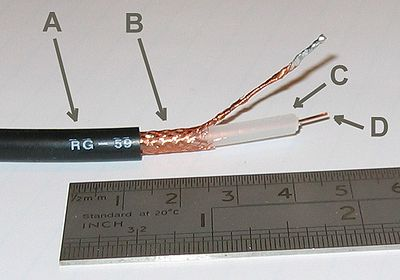
\includegraphics{images/400px-RG-59}
   % \caption{Kooksiyel Kablo}
    % \label{fig:kooksiyel_kablo}
  %\end{figure}


 \section*{AĞ TOPOLOJİLERİ }
%\begin{figure}[!ht]
%    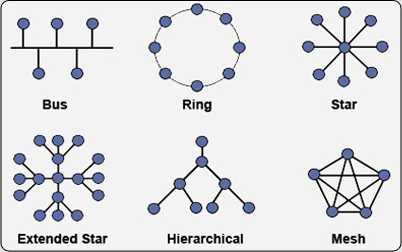
\includegraphics{../images/62_ağ_topolojisi.jpg}
%   \caption{Topolojiler}
%    \label{fig:topolojiler}
% \end{figure}
 % bu kısm notlarda yok topoloji nedir kısmını ben ekledim.
Ağ topolojileri nedir sorusunun en net cevabı, “bir ağı oluşturan cihazların fiziksel ve mantıksal yerleşimidir“.Network Topology (Ağ Topolojisi) Yerel Ağ Alanı (LAN) içerisinde bulunan bilgisayarların fiziksel ve mantıksal yerleşimini ifade eder. Fiziksel Topoloji ağ içerisinde bulunan tüm cihazların birbirlerine nasıl bağlanacağını ve bağlantı için ne tür kablo kullanacığını belirtirken Mantıksal Topoloji bu cihazların nasıl haberleşeceğini belirtir ve bu cihazları ortak bir protokol altında birleştirir. Kullanılmak istenen Ağ Teknolojisine göre farklı ağ topolojileri kullanılmaktadır.
Fiziksel Topolojinin 6 farklı çeşidi vardır. Bunlar Bus(Yol), Ring(Halka), Yıldız(Star), Ext Star(Gelişmiş Yıldız), Mesh(Örgü) ve Tree(Ağaç) topolojileridir. Broadcast(Yayın) ve Token Passing(İz) mantıksal topolojilere birer örnektir 

\subsection*{DOĞRUSAL (BUS) TOPOLOJİ}
Doğrusal bir hat üzerinde bilgisayarların T konnektörlerle bağlanması şeklinde kurulur.Hattın her iki ucunda 
sonlandırıcı kullanmak zorunludur.Kooksiyel kablo kullanılır.Ağın herhangi  bir noktasında arıza olması durumunda ağın tamamı çöker.Ağdaki veri trafiği tüm uçlara gider.
Herkes herkesin trafiğini görebilir.Bu yüzden çok fazla \textbf(çakışma(cooolision)) olur.
\begin{figure}[!ht]
    
\includegraphics{images/bus-topolojisi}
   \caption{Bus Topolojisi}
   \label{fig:bustopolojisi}
 \end{figure}

\subsection*{HALKA (RING) TOPOLOJİ}
Doğrusal topolojiye benzer.Sonlandırıcı kullanılmaz.Hattın iki ucu birleşiktir.
Hatta sanal  bir jeton dolaşır(token).Jeton sırası gelen bilgisayar,jeton boş ise göndereceği veriyi hatta yerleştirir.
Bilgisayarlar sırayla  veri gönderdiklerinden çakışma daha azdır.Günümüzde hiç kullanılmamaktadır.
Herkes herkesin verisini kullanabilmektedir.
%bu fotoğraf en alta geçiyor düzeltilecek
%\begin{figure}[!ht]
%    
\includegraphics{images/ring-topology-removebg-preview}
%    \caption{Halka-Ring Topolojisi}
%   \label{fig:halka_topolojisi}
%  \end{figure}
%

\subsection*{YILDIZ (STAR) TOPOLOJİ}
Merkezde dağıtıcı bir cihaz olur.Burdan tüm bilgisayarlara birer kablo gider.Ağın bir noktasındaki arıza sadece ilgili bilgisayarın ağ bağlantısına zarar verir.Genellikle \textbf(bükümlü çift (twisted pair,xtp)) kullanılır.Trafiğin herkese mi gönderileceği ya da sadece ilgili ucamı gideceği dağıtıcıya bağlıdır.
Dağıtıcının  performansı ve kabiliyeti ağı doğrudan  etkiler.
Günümüzde en yaygın topolojidir.
%YERİ DÜZELTİLECEK
%\begin{figure}[!ht]
%    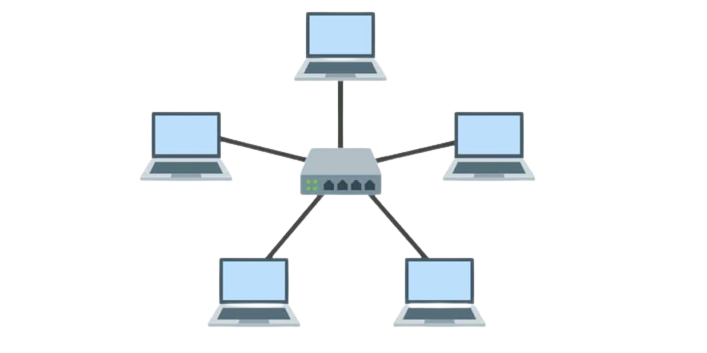
\includegraphics{images/star-Topology-1024x512-removebg-preview}
%    \caption{Yildiz-StarTopolojisi}
%   \label{fig:yildiz_topolojisi}
%  \end{figure}

\subsection*{ÖRGÜ (MESH)TOPOLOJİ}
%YERİ DÜZELTİLECEK
%\begin{figure}[!ht]
   % 
\includegraphics{images/mesh-topology-1-1024x512-removebg-preview}
    %\caption{Örgü-Mesh Topolojisi}
 %  \label{fig:Orgu_mesh_topolojisi}
  %\end{figure}
Uçları arasında birden fazla rota üzerinde haberleşme imkanı olan yapılardır.
Günümüzde genellikle farklı yıldız ağlar arasında yedekleme amacı olarak kullanılır.


\subsection{BÜKÜMLÜ ÇİFT KABLO}
  İçerisinde 4 çift bakır kablo bulunur.Kabloların birbireri üzerindeki direnç elektromanyetik etkisini azaltmak için ikişerli olarak sarılı durumundadırlar.
  Örneğin; UTP,CAT5,Ethernet Kablosu 
  %\begin{figure}[!ht]
  %  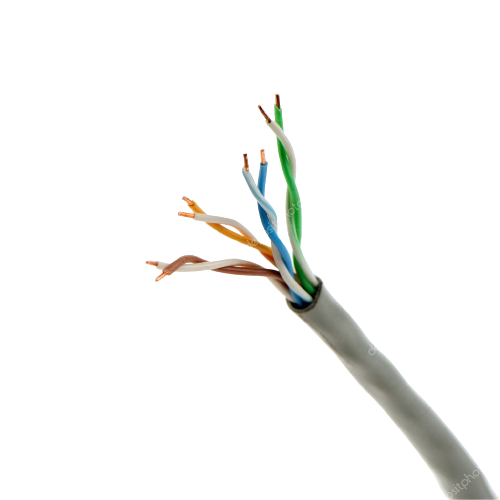
\includegraphics{images/bukumlukablo}
   % \caption{Bükümlü çift kablodan bir kesit}
 %\label{fig:Bukumlu_cift_kablo}
  %\end{figure}

\subsubsection{UTP(UNSHİLDED PWİSTED PAİR)Korumasız Bükümlü Çift} 
    8 iletkenin her biri ince bir yalıtkan ile kaplanmıştır.En dışında tamamını kaplayan bir yalıtkan vardır.
\subsubsection{STP(SHİLDED TWİSTED PAİR)} 
Her çiftin altında koruma (topraklama ) vardır.
\subsubsection{FTP(FOİLED TWİSTED PAİR )} 
4 çiftin tamamının etrafında folyo koruma vardır.
\subsubsection {S/FTP }
İkisininde özelliğini taşımaktadr.
    
\subsection{BANT GENİŞLİKLERİNE GÖRE(FREKNASLARINA)BÜKÜMLÜ ÇİFT KABLO}
\textbf{CAT:}\\
\textbf{CAT1-CAT3} \\
Telefon hatlarında bulunur.\\
\textbf{CAT5} \\
En yaygın kullanılan ağ kablosudur.Azami 100 m mesafe ve 10 m b/s destekler\\
\textbf{CAT6} \\
100 m mesafede 1G b/s destekler.\\
\textit{10 BASE T} Ethernet(Eth)\\
\textit{100 BASE T} Fast Ethernet(Fa,Fe)\\
\textit{1000 BASE T} Gigabit Ethernet(G,GE)\\
Bükümlü çift CAT5 VE CAT6 Kabloları  sonlandırmak için RJ-45 adı verilen connektörler kullanılır.
Bu kablolar iki farklı iki şekilde sonlandırılabilir.\textbf{568-A,568-B}\\
Kablonun iki ucunun aynı standarlarla sonlandırılmasna \textbf{Düz(Straight kablo )} denir.İki ucunda iki farklı standartta sonlandırılma yapılırsa \textbf{çapraz(cross-over)kablo } adı verilir.
\section{IP ADRESİ VE HESAPLAMALARI} %Notlarda 27.sayfa
32 bit uzunluğa sahip olan IP adresi 2 temel bileşene sahiptir. 

\begin{enumerate}
\item Ağ tanımlayıcı
\item Host tanımlayıcı
\end{enumerate}

\textbf{NOT : }Bir ağ içerisinde IP atanabilen ve kendisinin ağa bağlanma ihtiyacı olan bilgisayar, yönlendirici, güvenlik duvarı vb. cihazların tümüne host denir. 

IP adresinin bu iki bileşeni hesaplanırken alt ağ maskesine ihtiyaç duyulur. Temel olarak alt ağ maskesi IP adresinin sınıfına göre belirlenir. IP adresleri 32 bitin sekizerli olarak gruplandırılması ve decimal olarak gösterilmesi şeklinde olur. Bu 8 bitlik grupların her birine oktet denir. Her oktet birbirinden nokta ile ayrılır. 

\textbf{ÖRNEK : }
\begin{center}
\begin{tabular}{cccc}
00001010.&00000000.&00000001.&10000000 \\
10.       & 0.      & 1.      & 128      \\
Her sekizerli & & & \\
grup bir oktet & & &
\end{tabular}
\end{center}

Bir IP adresinin bağlı olduğu sınıf ilk oktetinden anlaşılır. 

\begin{center}
\begin{tabular}{cc}
00001010.00000000.00000001.&10000000 \\
ağ tanımlayıcısı           &  host tanımlayıcısı \\ 
24 bit ile $2^{24}$ tane ağ tanımlanabilir & 8 bit ile $2^8=256$ tane ağ tanımlanabilir\\
\end{tabular}
\end{center}

\textbf{ÖRNEK : } 16 tane IP adresini bölüyoruz. (${2^4}$ bit ) 

Görsel-1

\textbf{NOT : }Ağlardaki bilgisayar sayıları(kullanılabilecek ip sayıları) belirlenirken maksimum kapasite 2'nin kuvveti ${2^n}$ %katı yazılmıştı, kuvveti olarak değiştirdim
alınarak belirlenir. 

\textbf{ÖRNEK : }Bir şirketin iki farklı şubesinde 120 ve 280 adet bilgisayar kullanılmaktadır. Bu şirketler için optimal ağ büyüklüklerini hesaplayınız. 

\begin{itemize}
\item[]$120 => 2^n = 2^7 => 128$
\item[]$280 => 2^n = 2^9 => 512$
\end{itemize}

\textbf{NOT : }Host tanımlayıcısı kısmında belirtilen bitlerde elde edilebilecek en büyük sayı o ağda kullanılabilecek IP adresi sayısıdır. Her ağın ilk IP adresi \underline{"ağ adresi"} ve son IP adresi \underline{"yayın adresi"} olarak kullanıldığından her ağda kullanılabilecek host sayısı IP sayısından 2 eksiktir.
\begin{itemize}
\item[] Host bitleri : n tane 
\item[] Ağdaki IP adresi : $2^n$ tane 
\item[] Ağda kullanılabilecek host sayısı $2^n-2$
\end{itemize}

\textbf{ÖRNEK : } 10.9.8.0 IP adresinin 30. bitten sonrasının bulunduğunu varsayalım. Alt ağ IP adresinin kullanım amacına göre yazalım. 

\begin{tabular}{ll}
..... & ..... \\
30 bit& 2bit\\
\end{tabular}

IP sayısı $2^2=4$ tane
Host sayısı $2^2-2=2$ tane


\begin{tabular}{lll}
1.IP adresi 10.9.8.0 & ->& Ağ adresi \\
2. ve 3. IP adresi 10.9.8.1 ve 10.9.8.2 & -> & Hostlar için kullanılabilir \\
4. IP adresi 10.9.8.3 & -> & Yayın adresi 
\end{tabular}

\textbf{NOT : }

\begin{tabular}{ll|l}
Ağ sayısı & Host sayısı &Toplam host sayısı\\
\hline 
1&16&14 \\
2 & 8 & $2(8-2) =12$ \\
4&4&$4(4-2) = 8$ \\
\end{tabular}


\subsection{IP Sınıfları}
IP'nin ilk tasarlandığı sıralarda ortaya çıkmış bir kavramdır. Kurumlarda IP adresleri tahsis edilirken ihtiyaca göre optimal sayıda verebilmek için tasarlanmıştır. En büyük IP sınıfı A sınıfı, en küçük IP sınıfı C sınıfıdır. 

\underline{A sınıfı :} İlk biti(MSB) 0 olan IP adresleridir. 

\begin{tabular}{l}
01111111.11111111.11111111.11111111 \\
  127  \hspace{1.1cm} 255\hspace{1.1cm}255\hspace{1.1cm} 255 \\
\end{tabular}

İlk oktet 0-127 arasında olur. Varsayılan ap maskesi 255.0.0.0'dır. A sınıfı bir IP adresinde $2^{24}$ tane IP oluşturulabilir.

\underline{B sınıfı} İlk iki biti 1.0 şeklindedir. Ondalık formda ilk  okteti 128 ve 191 arasındaki adreslerdir. Varsayılan alt ağ maskesi 255.255.0.0'dır. B sınıfı bir IP adresinde $2^{16}$ tane IP oluşturulabilir.


\underline{C sınıfı} İlk üç biti 1.1.0 şeklindedir. Ondalık formda ilk okteti 192 ve 223 arasındaki adreslerdir. Varsayılan alt ağ maskesi 255.255.255.0'dır. B sınıfı bir IP adresinde $2^{8}$ tane IP oluşturulabilir.

\underline{D sınıfı} İlk dört biti 1.1.1.0'dır. Ondalık formda ilk okteti 224-239 arasındadır. \underline{Multicast}(Çoklu yayın) olarak bilinir. Normalde hostlarda kullanılmaz. 

\underline{E sınıfı} 240-248 ile başlar. Deneysel amaçlar için rezerve edilmiştir. Normalde hostlarda ve ağlarda kullanılmaz.

\begin{tabular}{lll}
A sınıfı & 0-127 & \\
B sınıfı & 128-191 & \\
C sınıfı & 192-223 & \\
D sınıfı & 224.0.0.0 \vline & Kullanmıyoruz \\
E sınıfı & 255.0.0.0 \vline  &Kullanmıyoruz \\
\end{tabular} 

Peki neden böyle bir sınıflandırma yapıldı?

\begin{tabular}{l|l|l}
Ağ biti & Host bitleri & Her ağdaki IP sayısı \\
\hline
8& 24->A sınıfı &$2^{24}$ tane IP \\
16& 16->B sınıfı &$2^{16}$ tane IP \\
24&8->C sınıfı &$2^8$ tane IP \\

\end{tabular}

\textbf{ÖRNEK : } 132.x.x.x IP adresi B sınıfıdır.
132.45.x.x IP adresinin ilk iki okteti ağ tanımlayıcısı son iki oktet host tanımlayıcısıdır. $2^16$ tane IP alabilir. 

112.x.x.x IP adresi A sınıfıdır. $2^{24}$ tane IP alabilir.

193.140.253.x IP adresi C sınıfıdır. $2^8$ tane IP alabilir.


\subsection{Özel IP Adresleri(Private IP Blocks)}

İnternette kullanılmayan IP adresleridir. İnternet üzerinde hiçbir yönlendirici tarafından yönlendirilmeyen IP adresleridir. Bu adreslerin kullanım amacı test uygulamaları ve NAT uygulamaları gibi durumlardır. IP adresleri tükendiğinden kurumlarda kullanılan bilgisayarların tamamına yetmemektedir. Bu nedenle günümüzde kurumların iç ağlarında özel IP adresleri istenilen sayıda kullanılabilir. 

\begin{itemize}
\item 10.0.0.0/8 ->$2^{24}$ IP adresi
\item 172.16.0.0 ->$2^{20}$ IP adresi
\item 192.168.0.0 ->$2^{16}$ IP adresi
\end{itemize}

\textbf{NAT(Network Address Translation)}

-Görsel NAT


\subsection{Ağ Maskesi(Netmask)}

IP adreslerinin bitlerden oluştuğunu ve iki bileşeni olduğunu biliyoruz. Bu iki bileşenin hangi bitten ayrılacağını bulmak için ağ maskesi kullanılır. Ağ maskesi herhangi bir IP adresi ile ikilik sistemde çarpılırsa(ve işlemi) çıkan sonuç ağın adresini verir. 


\textbf{ÖRNEK : }

\begin{itemize}
\item[] IP : 192.168.1.75
\item[] Ağ maskesi : 255.255.255.0
\item[] 11000000.10101000.00000001.01001011
\item[] 11111111.11111111.11111111.00000000
\item[] 11000000.10101000.00000001.00000000
\item[] Ağ adresi 192.168.1.0
\end{itemize} 

\subsection{CIDR Notasyonu}

Elimizde sadece IP adresleri olduğunda ağla ilgili yeterli bilgiye ulaşamadığımızı, ilave olarak IP adresinin hangi bitten bölündüğünü bilmemiz gerektiğini biliyoruz. Bunun için ağ maskesine alternatif olarak CIDR Notasyonu kullanılmaktadır. Bu gösterim şeklinde IP adresinin sağına "/" işareti konulup bölünen bit numarası yazılır. 

\textbf{ÖRNEK : } 

\begin{itemize}
\item[] 192.168.1.75 IP adresli ve 255.255.255.0 ağ maskesine sahip bir cihazın CIDR notasyonu 192.168.1.75/24 şeklindedir. 
\item[] 10.1.0.0 ve 255.0.0.0 ise 10.1.0.0/8 olarak gösterilir. 
\item[] 10.9.8.0 ve 255.255.255.128 ise 10.9.8.0/25 şeklinde gösterilir. (128 ikilik tabanda 10000000 şeklinde gösterildiğinden soldan 25 tane 0 vardır.) 
\end{itemize}

\subsection{Alt Ağa Bölme}
IP adresi ve ağı temsil eden bit sayısı belirli olan bir ağ birden fazla küçük ağlara bölünebilir. Alt ağa bölme işlemi alt ağ maskesinde bir bit kaydırılarak yapılır. Bu şekilde $2^n$ tane alt ağ bölme işlemi yapılabilir. 

\textbf{ÖRNEK : } 

\textbf{a)} 10.0.0.0/24 ağını iki ayrı ağa bölelim.



\textbf{b)}Yeni oluşturulan ağlar için 10.0.0.100 ve 10.0.0.150 IP adreslerinin aynı ağda olup olmadıklarını hesaplayın. (İpucu : Ağ adresi = IP x Ağ maskesi)

\textbf{c)}128 IP'li ağların her birini ikiye bölünüz. 


\underline{Çözüm :}

\textbf{a)}
\begin{itemize}
\item[] Ağ : 10.0.0.0/24
\item[] Ağ maskesi : 255.255.255.0 (24 tane 1 8 tane 0 var. $2^8$ tane IP var)
\item[] Ağ maskesi : 11111111.11111111.11111111.00000000 ağ maskesinde 1 bit sağa kaydırdığımızda 25 tane 1 7 tane 0 olacaktır. $2^7=128$ tane IP elde edilir. 
\end{itemize} 

1 bit kayarsa $2^1=2$ alt ağ
2 bit kayarsa $2^2=4$ alt ağ
\vdots
n bit kayarsa $2^n$ alt ağ elde edilebilir. 

10.0.0.0/25 notasyonuna sahip bir ağda 1.alt ağ 10.0.0.0 IP adresiyle başlar. 128 adet IP tanımlanır. Son IP 10.0.0.127 olur. 2. alt ağ ise 10.0.0.128 IP adresinden 10.0.0.255 IP adresine kadar 128 adet IP alabilir. 


\begin{tabular}{l|l|l|l|l|l}
&Ağ adresi & Yayın adresi & Ağ maskesi & IP sayısı & Host sayısı\\
\hline
1.ağ & 10.0.0.0/25 & 10.0.0.127 & 255.255.255.128 & 128 &126 \\
\hline
2.ağ & 10.0.0.128/25 & 10.0.0.255 &255.255.255.128 & 128 & 126 \\

\end{tabular}


\textbf{b)}

\begin{tabular}{llll}
& 00001001.00000000.00000000.01100100 &=& 10.0.0.100\\
ağ maskesi:& 11111111.11111111.11111111.00000000 &=&10.0.0.128\\
\hline
&00001001.00000000.00000000.10010110 &=&10.0.0.150 \\

\end{tabular}

Son oktetleri farklı olacağından aynı ağda değillerdir. 

\textbf{c)} 

\begin{tabular}{cc}
1.ağ & 2.ağ \\
\hline
10.0.0.0/25 & 10.0.0.128/25 \\
\end{tabular}

Ağ maskesi 255.255.255.128 

1111111.11111111.11111111.10000000

Yeni oluşan ağ maskesi 255.255.255.192

\begin{tabular}{ll}
1.ağ & \begin{tabular}{l}
10.0.0.0 ->ağ \\
\hline
10.0.0.63 ->yayın \\
\end{tabular}  \\   
\end{tabular}

\begin{tabular}{ll}
2.ağ & \begin{tabular}{l}
10.0.0.64 ->ağ \\
\hline
10.0.0.127 ->yayın \\
\end{tabular}  \\   
\end{tabular}



\begin{tabular}{ll}
3.ağ & \begin{tabular}{l}
10.0.0.128 ->ağ \\
\hline
10.0.0.191 ->yayın \\
\end{tabular}  \\   
\end{tabular}


\begin{tabular}{ll}
4.ağ & \begin{tabular}{l}
10.0.0.192 ->ağ \\
\hline
10.0.0.255 ->yayın \\
\end{tabular}  \\    
\end{tabular}

\textbf{SORU : } 10.9.6.0/25 ağını 4 ayrı ağa bölünüz.

Ağ maskesi 255.255.255.0
11111111.11111111.11111111.0

\begin{tabular}{lll}
Yeni ağ maskesi  & : &11111111.11111111.11111111.11100000 ($2^5=32$ IP var.) \\
                 & : & 255.255.255.224   \\
\end{tabular}

\begin{tabular}{ll}
10.0.0.0 & 10.0.0.64 \\
10.0.0.31 & 10.0.0.127\\
\end{tabular}









\section{IP YÖNLENDİRME}
\section{Bilgisayar Ağları Modelleme}
\subsection{Simülatör \& Emülatör}
Bilgisayar üzerinde bir ağı modellemek için; simülatör ve emülatör şeklinde iki tür program kullanılmaktadır:

\textbf{Simülatör}: Gerçek ortamdaki sistemler ile (çok benzese de) birebir aynı şekilde çalışmaz. Uçuş simülatörleri buna örnek gösterilebilir. Gerçek sistemlerde kullanılan donanımların üzerindeki yazılımlar bunda kullanılmaz, simülatörlerde kullanılan sanal cihazlarda özel geliştirilmiş ve kısıtlı yazılımlar çalışır. Ayrık zamanda çalışır: gerçek hayatta binlerce saat sürecek bir işlem 1 saniyede yapılabilir;  gerçek hayatta 1ms içerisinde biten bir eylem saniyelerce sürecek şekilde yavaşlatılabilir.

\vskip 0.5cm
\textbf{Emülatör}: Gerçek cihazlarda kullanılan yazılımlar doğrudan burada da çalıştırılır. Virtualbox üzerinde Windows çalıştırmak için, gerçek Windows kurulumu yaptığımızı hatırlayın. Donanımlar sanallaştırılır ama donanımlar üzerinde gerçek yazılımlar (işletim sistemleri) kullanılır. Gerçek zamanda çalışır.

\vskip 0.5cm
Simülatör ve emülatör kavramlarını bilgisayar ağları konusu özelinde özetlemeye çalışalım.
\vskip 0.5cm

İnternet'in ortak dilinin IP olması gibi, bilgisayar ağlarında ortak donanım da Cisco firmasının ürünleridir. Pazara erken girmiş olması, ürünlerinin kaliteli olması, geniş ürün yelpazesi olması, bol miktarda dokümanı olması, kullanıcı sayısının çok olması, vb. nedenlerle bilgisayar ağları çalışan hemen herkes Cisco cihazlara hakim olmaktadır. Bu nedenle, ağ modelleme programlarında öncelikle Cisco cihazlara (yönlendirici, anahtar, vb.) destek sağlanmaktadır.

Emülatör uygulamalarında, \textit{-simülatörlerden farklı olarak-} gerçek Cisco işletim sistemi kullanılması gerekmektedir. Gerçek işletim sistemi kullanıldığı için, gerçek cihazlarla yapılan fiziksel ağ uygulamalarına çok yakın bir çalışma ortamı sağlamaktadır. Bunun en büyük dezavantajı ise Cisco işletim sistemleri ücretli olduğu için ilave maliyet çıkarmasıdır. Diğer taraftan; bu işletim sistemlerinin İnternet'in yeraltı dünyasında yaygınlaşması gibi illegal durumlara da sebebiyet vermektedir.

\subsection{Ağ Modelleme Platformları (Ücretsiz Olanlar)}
\subsubsection*{Cisco Packet Tracer}
Cisco firması tarafından geliştirilmektedir. Cisco'nun Networking Academy adı altında vermiş olduğu eğitimlerde katılımcılara verilmektedir. Bunun haricinde satışı bulunmamaktadır. Simülatör tarzında bir uygulamadır.


\section{SONUÇLAR VE ÖNERİLER}

\section{EKLER}

\renewcommand{\refname}{KAYNAKLAR}
\addcontentsline{toc}{section}{KAYNAKLAR}
\shorthandon{=}
\end{document}
%